\chapter{Introduction}

% Organizational detail: AD and amyloid (which one should go first?). Center it on Amyloid, and then bring in AD as a central motivation for doing amyloid science.

% I think my focus should still be on Alzheimer's disease ... the practical purpose of my work is to understand how inositol works
% I am not trying to cure all amyloid diseases.
\section{Alzheimer's Disease}
% Here, my intention is to lead into the discussion of amyloid by giving a historical perspective and overview of AD
% And use AD as a motivation for why so much work has gone into studying amyloids.
\begin{outline}[enumerate]
	\1 More than a hundred years have pass since Dr. Alois Alzheimer first presented the connection between the presence of neuronal plaques and the clinical symptoms of presenile dementia characteristic of Alzheimer's disease (AD).

	\1 Today, AD is known to be the most common cause of dementia in persons of age 65 or older. With the increasing longevity of our population, AD is approaching epidemic proportions with no cures or preventative therapy available.\cite{Blennow:2006wd}

	% Elaborate on happened between the step above and the amyloid hypothesis?
	\1 The discovery of amyloid plaque deposits of the brains of deceased dementia patients led to the formulation of the amyloid hypothesis which posits that amyloid aggregates initiates the pathogenesis of AD, whereas the other pathological symptoms such as neurofibrillary tangles are secondary.

% \2 A$\beta$ is produced by intramembrane proteolytic cleavage of the larger amyloid-$\beta$ precursor protein (APP) by $\beta$-secretase, and is produced constitutively as part of the normal cellular metabolism.\{Selkoe, 2002 \#222\} Depending on the position of the cleavage, A$\beta$ peptides of lengths varying from 38 to 43 residues can be produced. However, the peptides spanning residues 1--40 (A$\beta$40) or 1--42 (A$\beta$42) are predominantly found AD-associated plaques.
\end{outline}

\subsection{Other amyloid diseases}
Many diseases have been identified to be linked with the presence of amyloid: Type II diabetes, Prion-related diseases, Parkinson's, Huntington's disease etc.


\section{Amyloid: formation and mechanism of toxicity}
  % In this section I will talk about how amyloid aggregation is thought to work. Introduce the thermodynamic model for understanding fibril formation. I will now broadly introduce to amyloid.  
  \begin{outline}[enumerate]
    \1 Although initial studies of amyloid was focused on understanding the etiology of AD, amyloid science now have grown into its own field.

    % \1 Finding a treatment for AD and other fatal neurodegenerative diseases motivated many biochemical and biophysical studies of the amyloid state.  
    \1 In the laboratory, a variety of proteins and peptides, both folded and disordered, have been shown to form amyloid fibrils via chemical modification of solution conditions and denaturation. It is currently thought that amyloid fibrillar state may be the globally stable folded state for all proteins.

    \1 Amyloid fibrils are formed via a complex aggregation pathway. Initially, monomers aggregate to form oligomers with different morphologies which exists in equilibrium with amyloid fibrils. Some of these oligomers are on-pathway to fibril formation, while others themselves may be end-points of the aggregation pathway. Amyloid fibrils, typically the visible endpoint of aggregation, has a cross-$\beta$ structure.
  \end{outline}

 \subsection{Structure of Fibril}
   \begin{outline}
    % \1 Add details on the definition of the cross-$\beta$ structure and its significance.
    \1 Decades after the initial discovery by Alois Alzheimer, A$\beta$, the central protein component of neuronal plaques, was synthetically produced in the laboratory. In vitro, A$\beta$ was found to precipitate out of solution almost immediately. 
  		\2 Describe the molecular structure of A$\beta$ amyloid fibrils
  			\3 Define the cross-$\beta$ structure [Show a schematic here].
  		\2 Briefly mention the techniques that can be used to obtain structural information of amyloid fibrils.
		\end{outline}

  \subsection{Structure of Non-fibrillar oligomers}
   Because many of the dynamic and disordered nature of oligomeric aggregates, the structure of oligomers have been challenging to obtain via experimental protein structural determination methods.
	
  \subsection{Kinetics}
  Amyloid fibrils have been observed to form via a nucleation-polymerization process. In the nucleation phase, energetic barriers of aggregation must be overcome to form the initial aggregation nucleus or seed.  Following nucleation, free monomers bind to the nucleated aggregates and polymerize into mature fibrils.\cite{Murphy:2002fe}
    
  \subsection{Toxicity}
  \begin{outline}
  	% Key question in the field: What is the toxic species?
  	\1 Multiple lines of research have identified oligomers as a likely causative agent for neuronal cell death. By contrast, the monomeric and fibril forms are thought to be less toxic than oligomers. It is hypothesized that soluble oligomers may cause toxicity by perturbing the integrity of cellular membranes through binding and disrupting the lipid bilayer (perhaps by making them ion permeable). \cite{Walsh:2007fu}
  	\1 Include a paragraph about amyloid formation and lipid membranes (?)
  	% Understanding the toxicity or finding out whether there is a toxic species in part validates the amyloid hypothesis. 
  \end{outline}


\section{Amyloid Inhibition: A promising treatment for amyloid disorders}
% Cure, method of prevention; is there hope?
\begin{outline}
	\1 In this section, I will provide an overview of some of the challenges to overcome when developing a small molecule therapeutic for Alzheimer's disease.  Furthermore, using this information, I will motivate why inositol is an exciting avenue to explore.
	
	  \2 scyllo-Inositol is able to cross the blood brain barrier. It has high bioavailability. Because it is not broken down in the gut, it can be taken orally.
	  
	  \2 Inositol is not toxic to the human body.  Inositol is used in signaling pathways.

	\1 Briefly mention non-small molecule putative therapies which also acts via amyloid inhibition. The focus of this thesis will be on small-molecule amyloid inhibition.
\end{outline}

\subsection{Molecular mechanisms of amyloid inhibition 
            \\ by small molecules}
\begin{outline}[enumerate]
    \1 Amyloid inhibition as a treatment for Alzheimer's disease and related amyloid disorders. Amyloids are attractive drug targets. Small molecules may be one effective way to develop a treatment for amyloid disorders because they have the potential to be able to treat the underlying disease. Through in vitro screening, many small molecules have been found to effect the amyloid aggregation pathway.  Some were demonstrated to inhibit amyloid fibrils, where as others were shown to arrest or reduce oligomer formation.   
      % Here I can take a cue from Justin Lemkul`'s recent review paper.
      % Talk about the different kinds of small molecules that have been found to inhibition amyloid formation.  Here I will also provide a summary of what people know about the mechanism by which they inhibit amyloid formation.
      
      \2 Pharmacological perspective of the challenge of developing an Alzheimer's drug. In order to effectively treat Alzheimer's and other neurodegenerative diseases, small molecule drug candidates must pass the blood brain barrier at sufficient concentrations for inhibition.  This is difficult to achieve.
      
      \2 In vitro screening has led to the discovery of a large number of small-molecules which were found to affect the amyloid aggregation pathway. Many of these small molecules are thought to act by directly binding to amyloidogenic peptides and aggregates.

      \begin{figure}
        \centering
        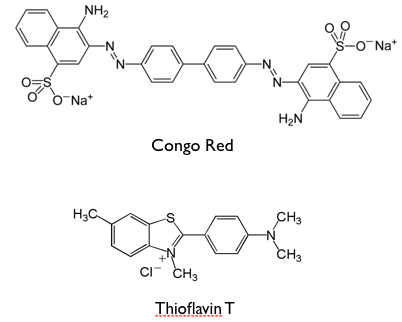
\includegraphics[width=3in]{figures/introduction/dyes.png}
        \caption[Small molecule binders]{Amyloid binding dyes Congo Red and Thioflavin T}
        \label{fig:amyloid_dyes}
      \end{figure}
            
        \3 Thioflavin T and Congo red are dye molecules used to identify the presence of amyloid.  Both molecules bind to mature amyloid fibrils and have been shown to affect fibril formation. Figure~\ref{fig:amyloid_dyes}

        \begin{figure}
          \centering
          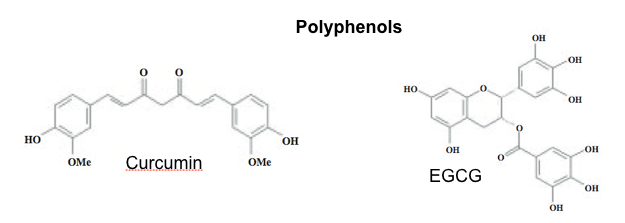
\includegraphics[width=6in]{figures/introduction/polyphenols.png}
          \caption[Small molecule binders]{Polyphenols}
          \label{fig:polyphenols}
        \end{figure}
        
        \3 Polyphenols is a large group of natural and synthetic molecules.  (−)-epigallocatechin-3-gallate, curcumin, and a polyphe- nolic grape seed extract are some that was found to inhibit fibril formation. Are also known for their anti-oxidant properties. Figure~\ref{fig:polyphenols}
      
      \2 Small molecule inhibitors share common chemical features and groups.  They are typically planar in geometry, have many aromatic rings, and polar functional groups (hydroxyl groups) around the edge of these aromatic rings.
    
    	\2 Mechanism of action. Some small molecules inhibit fibril formation, where as others may prevent oligomerization, but not fibrillation. A high concentration is often required to observe activity (micromolar to millimolar), which suggests that they may be non-specific inhibitors. EGCG, one such polyphenol, is known to have the lowest/highest IC50.
    	% IC50 -- This quantitative measure indicates how much of a particular drug or other substance (inhibitor) is needed to inhibit a given biological process (or component of a process, i.e. an enzyme, cell, cell receptor or microorganism) by half.
      % EC50 -- The term half maximal effective concentration (EC50) refers to the concentration of a drug, antibody or toxicant which induces a response halfway between the baseline and maximum after some specified exposure time.[1] It is commonly used as a measure of drug's potency.
      % Ref: wikipedia
      
      % Review of what is known about amyloid fibril ligand binding, specifically dyes.	
	    \3 Molecular mechanism of binding of dye molecules. Two types of binding modes. Bind flat on amyloid surface. Interact with hydrophobic groups exposed on the amyloid fibrils. Doesn't explain why the dye molecules are also able to suppress fibril formation.
      % Can the birefringence be explained by these binding modes? -- this is out of the scope of my thesis.  Don't put this in my thesis but I should be able to coherently explain this during my defense.
      
	\1 Inositol molecules
	
	\begin{figure}
    \centering
    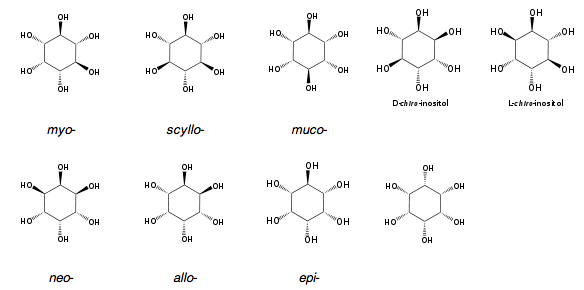
\includegraphics[width=6in]{figures/introduction/inositol.png}
    \caption[Inositol]{Inositol stereoisomers}
    \label{fig:inositols}
  \end{figure}
  
		\2 The discovery of inositol
		
		\2 Role of inositol in the human body 
		
			\3 \emph{myo}-inositol
			
		\2 Where is inositol found. Human body tissues. Myo- is present in certain grains, grape fruit but scyllo- is only found in small quantities in food sources.
		
		\2 Role of inositol in amyloid inhibition
		
			\3 in vitro studies
			
			\3 in vivo studies
\end{outline}

\subsection{Analogy to Sugar-protein binding}
% Does this section fit here? Where should I put it?
\subsubsection{Experimental techniques to study sugar-binding modes}
\subsubsection{Sugar Binding modes}


\section{Structure-based Drug Discovery}
\subsection{Forces in protein-ligand interactions}
\begin{outline}
	\1 Protein-ligand non-covalent interactions which are important for binding and recognition.
		\2 Electrostatic interactions: Polar and charge-charge interactions
			\3 Hydrogen bonding
			   % Here, it will benefit me to read Sarah's appendix C carefully.
		\2 Nonpolar (hydrophobic) interactions
		  \3 Van der Waals
\end{outline}

\subsection{Protein-Ligand binding}
% subsection protein_ligand_binding_theory (end)
% Below is a summary of an excerpt from Tom's thesis on structure-based drug discovery.
% Design of antibiotics 
% 1) Target determination (biochemical)
% 2) Structural determination (Xray, NMR, or homology); active site identified; Here would be useful to get the holo structure of the protein
% 3) Screen for inhibitors against a chemical library or in silico docking.
\begin{outline}
	\1 Enzyme and the ligand must bind tightly and specifically, so to avoid large drug doses to inhibit the enzyme, which may have adverse side effects (toxicity) in the human body.

	\1 Binding constant is a measure of the affinity of a ligand to a protein. It is the concentration at which 50\% of the drug is bound to the protein. In experimental studies, $K_d$ is often used to quantitatively identify potential binders. A small $K_d$ suggests that the ligand may bind tightly to the protein.

	\1 Binding equilibrium

    \begin{equation}
      \left[ Protein\cdot Inositol \right] 
      \rightleftharpoons 
      \left[ Protein \right]+\left[ Inositol \right]
    \end{equation}
  
    % \2 Absolute binding free energy
    % \2 Relative binding free energy
    
	\1 The binding free energy of a ligand to a protein is directly related to its dissociation constant, $K_d$, the equilibrium constant of the above reaction

     \begin{equation}
        K_{d} = f_{ub}\frac{\left[ Protein \right]\left[ Inositol \right]}{\left[Protein \cdot Inositol\right]},
     \end{equation}
     
	\1 Experimental techniques for estimating $K_d$
		\2 What experimental techniques are used to estimate binding affinity? (Study up on this.)
		\2 Isothermo-calorimetry (ITC) can be used to measure binding to peptides.
\end{outline}	

% \subsection{Role of chirality in drug binding}
% Stereoisomerism is important to the activity of molecules.  It modulates binding to proteins.
% Two types of stereochemistry
% Constitutional isomers - differs in bonding sequences and connectivity
% Stereoisomers - differs in orientation of their atoms in space, but no connectivity differences.
% Definition of chirality [Add schematic] ... etc
% Molecules with chirality have a non-superimposable mirror image, called an enantiomer.
% A carbon molecule with four different groups has chirality.
\addcontentsline{toc}{section}{Bibliography}
\bibliographystyle{plain}
\bibliography{chapter1}